\documentclass{article}
\usepackage{graphicx}
\usepackage[margin=1.5cm]{geometry}
\usepackage{amsmath}

\begin{document}

\title{Warm-Up Day 5}
\author{Prof. Jordan C. Hanson}

\maketitle

\section{More on Histograms}

\begin{figure}[ht]
\centering
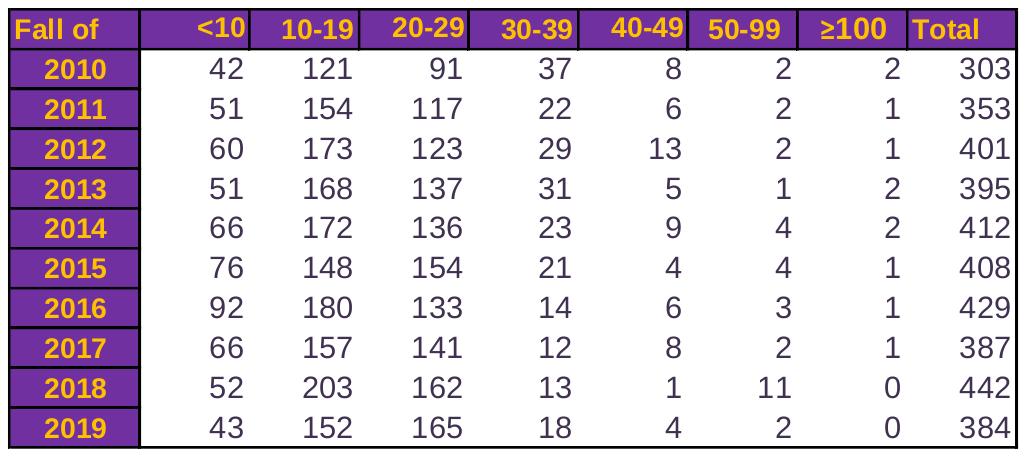
\includegraphics[width=0.55\textwidth]{class_size.png}
\caption{\label{fig:classsize} A listing of average class sizes for Whittier College for the past decade.}
\begin{enumerate}
\item Make a histogram of the class sizes for the year 2010 using the bins given by the purple headers ($<10,~10-19,...$). Normalize the histogram. \\ \vspace{3.5cm}
\item Repeat the first exercise for the year 2019. \\ \vspace{3.5cm}
\item Plot the two normalized histograms on the same set of axes.  What is the average class size for 2010 and 2020?
\end{enumerate}
\end{figure}

\end{document}
